% ---------------------------------------------------
% ----- Chapters of the template
% ----- for Bachelor-, Master thesis and class papers
% ---------------------------------------------------
%  Created by C. Müller-Birn on 2012-08-17, CC-BY-SA 3.0.
%  Freie Universität Berlin, Institute of Computer Science, Human Centered Computing. 
%
\chapter{Theoretical background}
\label{chap:background}

Before discussing the design and implementation of the UI editor, it is necessary to provide a brief overview of the applied parts of HCI and the specific context, challenges and Opportunities in which the UI editor was developed.
% 

\section{HCI}
Let me start by concretizing the HCI aspects and why this thesis approaches the area from an not so common standpoint.
\\
Many HCI books (e.g. \cite{Interactiondesign:2019ys} or \cite{LearnHCI:2020ys}) implicitly assume \label{def:Greenfield} Greenfield development,
which ''[...] is in its most distinct form when a new product is created from scratch – a new product or product platform, based on new technology, using new methodology [...]'' \cite{BrownfieldToGreenfield:2021ys}.
\\
While \cite[p. 392]{Interactiondesign:2019ys} for example mentions \textit{Environmental requirements} and \textit{Technical requirements} as part of the requirement discovery, the descriptions of these terms are more focused on physical limitations or user behaviours and technical requirements are mentioned only once and then not discussed further.
In contrast, I set my focus on the development inside a software company and an existing ecosystem, where resource, time and API limitations are present and existing users need to get productive with new software quickly.
\\
Thus, the user research phase started with collecting information about diffrent exisitng users as well as potentially new user groups the editor should target and adapting common HCI methods for qualtitative and quantitative user research like Moderated observations, interviews and questionaires.
I approached this phase with an open mind, recognizing that individual methods or applications of them might not be successful or don't provide value in this case study, but that much can still be learned from such experiences. As an example, after evaluation and test runs, I decided against Questionaires, because they showed less information content than other methods in this case study.
To align the methods with the projects goal and to select methods worthwhile trying from the large pool of user research methods, I used two systems:
\\
SMART criteria, which is a popular machanism to formulate goals and objectives that are clearly defined and also realistic to be implemented in time. \cite*{Atlassian:2021}.
I'll introduce them more in detail in chapter \ref*{chap:research}.
The second one are ''three major factors that an HCI designer should consider'' \cite[pp. 37-41]{LearnHCI:2020ys} according to Becker, which are
\begin{description}
  \item[Usability Factor] describes the spectrum from ''usable'' to ''unusable'' software. This is determined through the software design features implemented and how they help the user archieve their tasks in the environment provided.
  \item[Accessibility Factor] is high when as many users from different backgrounds can use the software in different enviornments. It includes, but is not limited to access for people with physical and other disabilites, as well as the entry hurdle a new user must overcome.
While it might look like this factor is not as important as the other two for specialized software mostly used internally, it should not be left out when designing and implementing. For example, even if currently no user with visual impairment is working with the software, it can always happen that an exisitng or new colleague suddenly has to rely on screen readers to continue his work.
  \item[Time-On-Task Factor] refers to ''[...] solutions that use up the appropriate of time to solve a problem.'' \Cite[p. 40]{LearnHCI:2020ys}. Obviously, to save users as much time as possible, a fast system is required.
But it is inevidable that the system, network delay and complexity of computation all have some minimal required time, and users understand that some operations might take time. More important is to reduce the perceived lag of interactions and give users feedback if a task takes longer to complete.
\end{description}
Evaluationg the outcomes of the research is at least as important as the research itself.
I experimented with diffrent ways to prepare and process the data to to present it more clearly as well as to consider different factors when discussing how to progress with the prototype.

\section{Project specific background}
To understand the usecase and value of the UI Editor, we first have to declare the fundamentals of the environment the editor will be embedded in.
The publishing houses resp. their digital departments (in the following \textit{customer}) purchase the license for an app or website (in the following just \textit{app}, as there is not much difference besides the end medium).
Then, they can import content via multiple ways into the system, or the editors write the content directly inside the tools provided as an Software-As-A-Service (SaaS).

\begin{figure}[h]
  \caption{Use Case diagram showing interactions from publishers, readers and frontend developers with the system}
  \includegraphics[width=\textwidth]{pics/purple-abstract.drawio.png}
\end{figure}

The UI editor fits into the Use case ''Per App configuration \& style'', with wich mostly Frontend Developers and Project Managers from Sprylab as well as some external customer's IT admins will interact. The goal is to lower the editing burden as much as possible, so that more of the configuration can be handed off to external customers while also improving usability for the developers of the company.
\\
Now that we have established a rough understanding of the environment and usecase the UI editor will be placed in, I want to explain more about the configuration and styling itself.
For that, it is important to understand the Frontend framework Sprylab uses for the delivery to apps and websites. It is called Purple Experience and is a Meta framework build ontop of Angular. The benefit is, that it is completely configurable via JSON files describing the routing, rendering of diffrent components,
connecting data sources (an API abstraction) with those components, loading assets like images and ads, and styling the whole page with CSS.
\\
These configs and assets are stored on an file system called \label{def:DynamicResources} \textit{dynamic resources}.
\\\\
Dynamic resources are individually managed and loaded for every app. This way, on mobile phones the endusers download an native core app, which in turn just downloads the dynamic resources and executes the angular app with the configs provided from the resources.
Similar, when a end user requests a website, the backend server just looks up the dynamic resources matching this app's Domain and renders the website using that config.
This way, all customers can share the same server instance(s), or at least don't require extra build artefacts per app.
\\
In addition, there are preview and live resources for every app, so that changes can be tested before they are released to the end users.
\\
If you have worked with larger, deeply nested JSON files before, you may recall that they get convoluted quite fast.
Also, manually handling ZIP files, changing assets and config files, packing everything back in a zip file and hoping one didn't introduce a typo anywhere is an inefficient an at times quite dangerous workflow.
\\
At Sprylab, there exists an tool called ''Storefront Editor'', which is used as the foundation for this new editor.
In the chapter \ref{chap:research} about User Research, I will outline the positive aspects and approaches which I reused for the new editor,
as well show the missing features and features the interview candidates noted as confusing, not working or slowing down their work.

The following UML sequence diagram displays a typical interaction of a user with the editor; pulling the current version, editing a file and merging the changes.
\textbf{TODO move to architecture?}
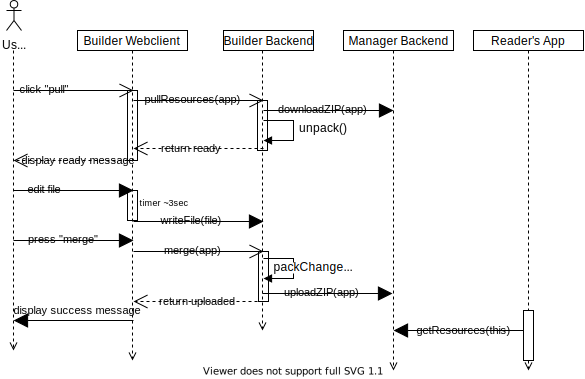
\includegraphics[width=\textwidth]{pics/user-flow.uml.drawio.png}